\documentclass{beamer}
\mode<presentation>
\usetheme{CambridgeUS}
\usepackage[russian]{babel}
\usepackage[utf8]{inputenc}
\usepackage[T2A]{fontenc}
\usepackage{sansmathaccent}

\usepackage{verbatim}
\usepackage{alltt}

\pdfmapfile{+sansmathaccent.map}
\title[Язык C]{Основы программирования на С, часть 4}
\author{Наумов Д.А., доц. каф. КТ}
\date[12.09.2019] {Операционные системы и системное программное обеспечение, 2019}

\begin{document}

%ТИТУЛЬНЫЙ СЛАЙД
\begin{frame}
  \titlepage
\end{frame}
  
%СОДЕРЖАНИЕ ЛЕКЦИИ
\begin{frame}
  \frametitle{Содержание лекции}
  \tableofcontents  
\end{frame}

\section{Интерпретация сложных деклараций}
\begin{frame}{Указатели на функции}
В языке Си можно определять указатели на функции, которые
ничем не отличаются от обычных указателей. 

\textbf{Например}: double (*fp)(double);

Указатель на функцию можно:
\begin{itemize}
\item присваивать, 
\item размещать в массиве, 
\item передавать в функцию в качестве параметра...
\end{itemize}
\begin{figure}[h]
\centering

\includegraphics[scale=0.6]{images/lec04-pic01.png}
\end{figure}
\end{frame}

\begin{frame}{Передача функции как параметра}
\begin{figure}[h]
\centering
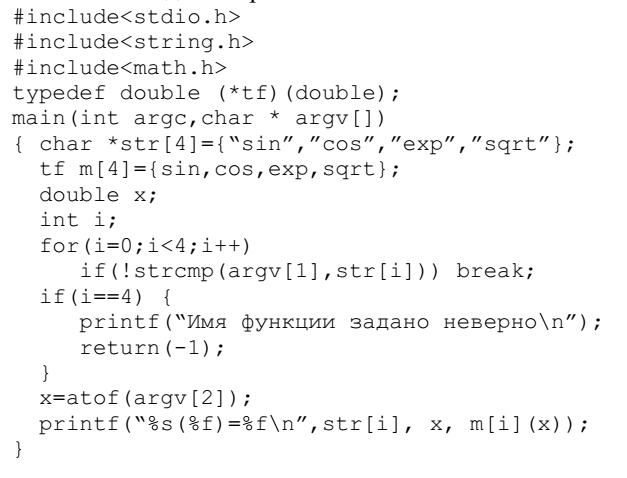
\includegraphics[scale=0.5]{images/lec04-pic02.png}
\end{figure}
\end{frame}

\begin{frame}
В декларациях обычно используется имя (идентификатор) и один из модификаторов *, [ ] и ( ), причем разрешается использовать более одного модификатора в одной декларации. 

Для раскрытия этих деклараций применяются следующие правила:
\begin{enumerate}
\item Чем ближе модификатор стоит к идентификатору, тем выше его приоритет.
\item Приоритет ( ) и [ ] выше, чем приоритет *.
\item Приоритет повышается заключением в скобки ().
\end{enumerate}
\begin{figure}[h]
\centering
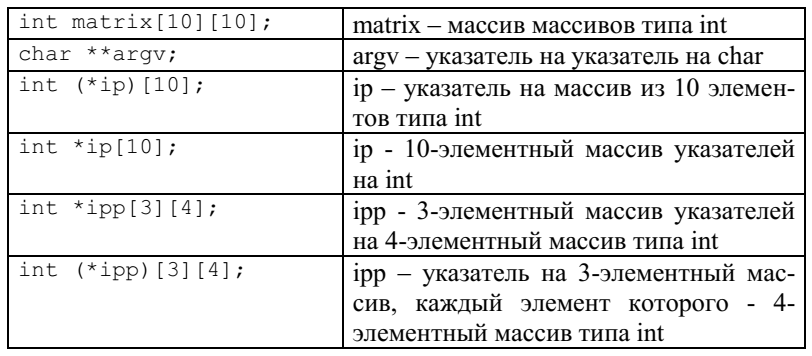
\includegraphics[scale=0.5]{images/lec04-pic04.png}
\end{figure}
\end{frame}

\begin{frame}
\begin{figure}[h]
\centering
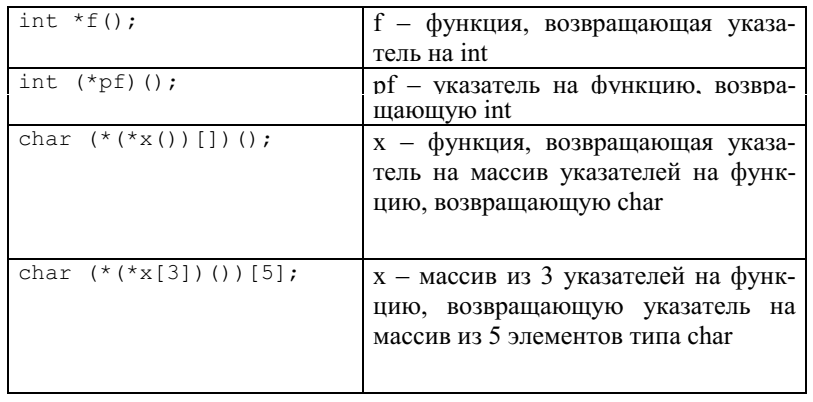
\includegraphics[scale=0.5]{images/lec04-pic05.png}
\end{figure}
\end{frame}

\begin{frame}{Оператор typedef}
Для упрощения прочтения сложных деклараций, а также для именования, типам данных можно задавать новые имена с помощью оператора typedef. 
\begin{itemize}
\item typedef double (*PFD)() - определяет тип PFD как указатель на функцию, возвращающую double.
\item оператор typedef не создает новый тип, а декларирует новое имя (синоним) уже существующего типа.
\end{itemize}
После ключевого слова typedef следует конструкция, синтаксически аналогичная блоку описания переменных, с той лишь разницей, что вводимое ею новое имя или имена являются не именами переменных, а новыми именами типов.

\textbf{Пример}: $typedef int number, * num\_pointer$;

\begin{itemize}
\item $number$ - синоним типа $int$;
\item num\_pointer - синоним указателя на $int$.
\end{itemize}
\end{frame}

\section{Структуры и объединения}

\begin{frame}{Декларация структуры}
Структура – это тип данных, позволяющий сгруппировать несколько переменных (возможно различного типа) под одним именем. 

В общем случае декларация структуры имеет следующий вид:
struct[<тег структуры>]{<список деклараций полей>};
\begin{figure}[h]
\centering
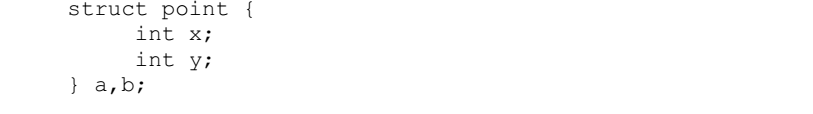
\includegraphics[scale=0.5]{images/lec04-pic06.png}
\end{figure}
Язык Си поддерживает именную, а не структурную, типизацию, что означает, что два неименованных структурных типа, пусть и содержащие совершенно идентичные списки деклараций полей, будут считаться различными и не будут совместимы по присваиванию.
\end{frame}

\begin{frame}{Декларация структуры}
\begin{itemize}
\item typedef struct point { int x; int y; } sp;
\item инициализация полей - struct point k = {3,5};
\item доступ к полям - k.x, k.y
\item p=\&k; p->x=2;
\end{itemize}
\begin{figure}[h]
\centering
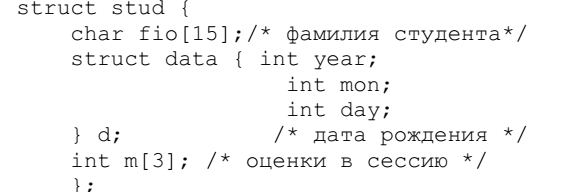
\includegraphics[scale=0.6]{images/lec04-pic07.png}
\end{figure}
\end{frame}

\begin{frame}
В Си разрешается присваивать и копировать структуры, что позволяет передавать их в функцию в качестве аргумента и передавать из функции в качестве возвращаемого значения (в отличие от массивов, структуры при этом копируются целиком), но структуры нельзя сравнивать. 
\begin{figure}[h]
\centering
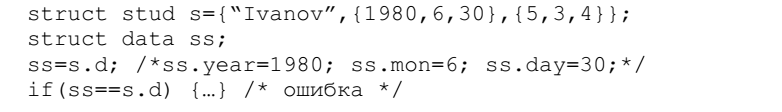
\includegraphics[scale=0.6]{images/lec04-pic08.png}
\end{figure}
\end{frame}

\begin{frame}
Написать функцию, параметрами которой являются массив анкет студентов (struct stud) и их количество. Функция печатает фамилии отличников и даты рождения.
\begin{figure}[h]
\centering
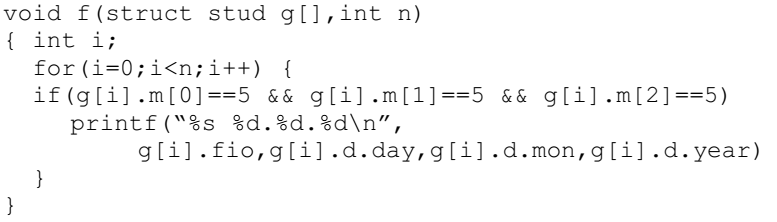
\includegraphics[scale=0.6]{images/lec04-pic09.png}
\end{figure}
\end{frame}

\begin{frame}{Размещение структуры в памяти}
\begin{figure}[h]
\centering
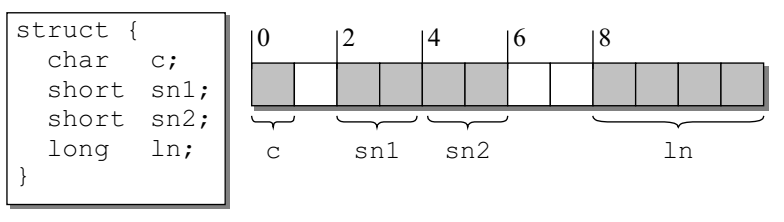
\includegraphics[scale=0.6]{images/lec04-pic10.png}
\end{figure}
Определить размер структуры - sizeof()
\end{frame}

\begin{frame}{Объединения}
\textbf{Объединение} (union) – это тип данных, позволяющий хранить разнородные данные (поля) в одной и той же области памяти. 
\begin{figure}[h]
\centering
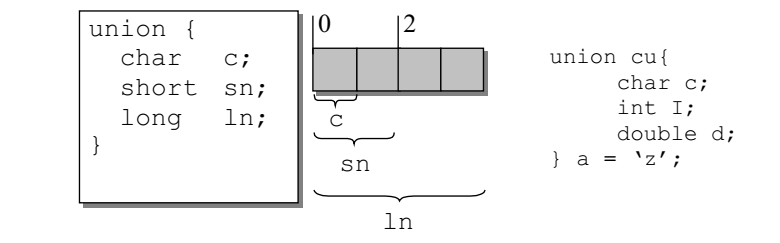
\includegraphics[scale=0.6]{images/lec04-pic11.png}
\end{figure}
\end{frame}

\section{Работа с динамической памятью}
\begin{frame}{Выделение памяти}
Для выделения памяти используется функция malloc из стандартной библиотеки.
\begin{figure}[h]
\centering

\includegraphics[scale=0.6]{images/lec04-pic12.png}
\end{figure}
\begin{itemize}
\item функция выделяет блок памяти указанного (в байтах) размера и
возвращает указатель на него;
\item тип size\_t представляет собой один из базовых целочисленных типов, размера которого достаточно для представления любого допустимого в данном контексте значения.
\item функция возвращает нетипизированный указатель,
перед использованием его, как правило, необходимо привести к требуемому типу.
\item в случае неудачи функция возвращает нулевой указатель.
\end{itemize}
\end{frame}

\begin{frame}{Освобождение памяти}
Для освобождения памяти используется функция free уиз стандартной библиотеки.
\begin{figure}[h]
\centering

\includegraphics[scale=0.6]{images/lec04-pic13.png}
\end{figure}
\begin{itemize}
\item функции должен быть передан указатель на начало блока памяти,
ранее выделенного с помощью malloc(). 
\item После обращения к free() этот указатель становится недействительным.
\end{itemize}
\end{frame}

\begin{frame}{Изменение размера блока памяти}
Для освобождения памяти используется функция realloc уиз стандартной библиотеки.
\begin{figure}[h]
\centering

\includegraphics[scale=0.6]{images/lec04-pic14.png}
\end{figure}
\begin{itemize}
\item функция при необходимости может выделить новый непрерывный блок динамической памяти требуемого размера, при этом она корректно скопирует туда содержимое старого блока и ос вободит старый блок памяти. 
\item функция возвращает новый указатель на блок измененного размера или, в случае неудачи, NULL (в последнем случае старый блок остается нетронутым). 
\item После обращения к realloc() старый указатель становится недействительным.
\end{itemize}
\end{frame}

\begin{frame}
Написать фрагмент программы, размещающий в динамической памяти вводимые из стандартного входного потока вещественные числа. Количество вводимых чисел вводится первым.
\begin{figure}[h]
\centering
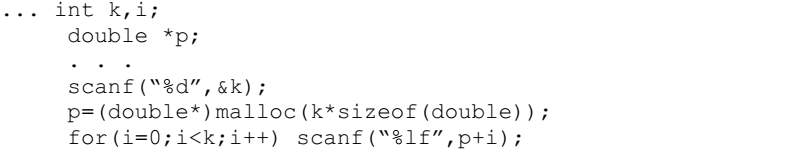
\includegraphics[scale=0.6]{images/lec04-pic15.png}
\end{figure}
\end{frame}

\begin{frame}
Ввести строку из стандартного входного потока длиной не более ста символов и разместить ее в динамической памяти.
\begin{figure}[h]
\centering
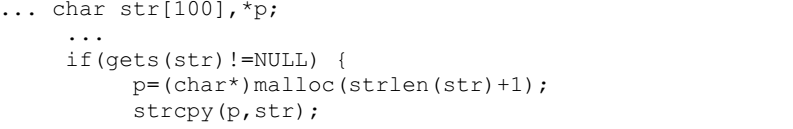
\includegraphics[scale=0.6]{images/lec04-pic16.png}
\end{figure}
\end{frame}

\begin{frame}
Ввести строку символов из стандартного входного потока и распечатать ее в обратном порядке, построив при этом в динамической памяти стек.
\begin{figure}[h]
\centering
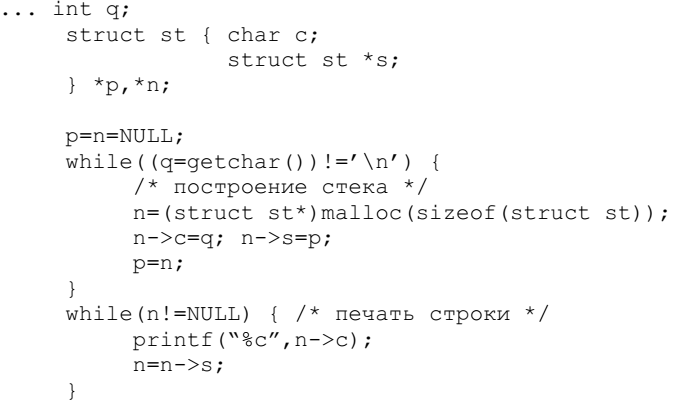
\includegraphics[scale=0.6]{images/lec04-pic17.png}
\end{figure}
\end{frame}

\end{document}
